% Thesis Figure 5.5: mean accuracy of HGANN-Mal against the majority baseline, GraphSAGE and
% HGNN+. Redraws the author-supplied chart (supplied/fig3-acc-dif.pdf) at text width, with the
% method colours of Figure 5.4. Keep these values aligned with Tables 5.1 and 5.2 in
% content/hgann-mal.tex.
\documentclass[border=1pt]{standalone}
\usepackage[T1]{fontenc}
\usepackage{textcomp}
\usepackage{tgheros}
\renewcommand{\familydefault}{\sfdefault}
\usepackage{tikz}

\definecolor{tumblue}{HTML}{0065BD}
\definecolor{tumblueii}{HTML}{64A0C8}
\definecolor{tumgrey}{HTML}{808080}
\definecolor{tumgreylight}{HTML}{CCCCCC}
\definecolor{tumgreydark}{HTML}{333333}
\colorlet{majority}{tumgreylight!55}
\colorlet{hgannmark}{tumblue!65!black}

\newcommand{\labelfont}{\fontsize{6.2}{7.1}\selectfont}
\newcommand{\valuefont}{\fontsize{6.0}{6.9}\selectfont\bfseries}
\newcommand{\axisfont}{\fontsize{6.0}{6.9}\selectfont}
\newcommand{\taskfont}{\fontsize{6.6}{7.6}\selectfont\bfseries}
\newcommand{\resultfont}{\fontsize{7.6}{8.7}\selectfont\bfseries}

% An accuracy of 0 lies at x = 40 mm and one of 100 at x = 110 mm. The two result columns are
% centred at x = 120 mm and x = 134.6 mm.
\newcommand{\accx}[1]{40+#1*0.70}

% #1 row centre, #2 task, #3 corpus, #4 majority, #5 GraphSAGE, #6 HGNN+, #7 HGANN-Mal,
% #8 HGANN-Mal minus HGNN+ as printed.
\newcommand{\accrow}[8]{%
  \pgfmathsetmacro{\xmaj}{\accx{#4}}%
  \pgfmathsetmacro{\xsage}{\accx{#5}}%
  \pgfmathsetmacro{\xplus}{\accx{#6}}%
  \pgfmathsetmacro{\xmal}{\accx{#7}}%
  \node[anchor=base east,inner sep=0pt] at (38,#1+0.6) {\taskfont #2};
  \node[anchor=base east,inner sep=0pt,text=tumgrey] at (38,#1-2.6) {\labelfont #3};
  \fill[majority] (40,#1-2.5) rectangle (\xmaj,#1+2.5);
  \fill[tumblueii] (\xmaj,#1-2.5) rectangle (\xsage,#1+2.5);
  \fill[tumgrey] (\xsage,#1-2.5) rectangle (\xplus,#1+2.5);
  \pgfmathparse{#7>#6 ? 1 : 0}%
  \ifnum\pgfmathresult=1
    \fill[tumblue] (\xplus,#1-2.5) rectangle (\xmal,#1+2.5);
  \fi
  \draw[hgannmark,line width=0.6pt] (\xmal,#1-3.4) -- (\xmal,#1+3.4);
  \node[inner sep=0pt] at ({(40+\xmaj)/2},#1) {\valuefont #4};
  \node[anchor=east,inner sep=0pt,text=white] at (\xsage-0.8,#1) {\valuefont #5};
  \node[anchor=south,inner sep=0pt,text=tumgreydark] at (\xplus,#1+3.9) {\valuefont #6};
  \node[inner sep=0pt] at (120,#1) {\resultfont #7};
  \node[inner sep=0pt,text=hgannmark] at (134.6,#1) {\valuefont #8};
}

\newcommand{\legenditem}[4]{%
  \fill[#3] (#1,#2-1.6) rectangle (#1+3.2,#2+1.6);
  \node[anchor=west,inner sep=0pt] at (#1+4.4,#2) {\labelfont #4};
}

\begin{document}
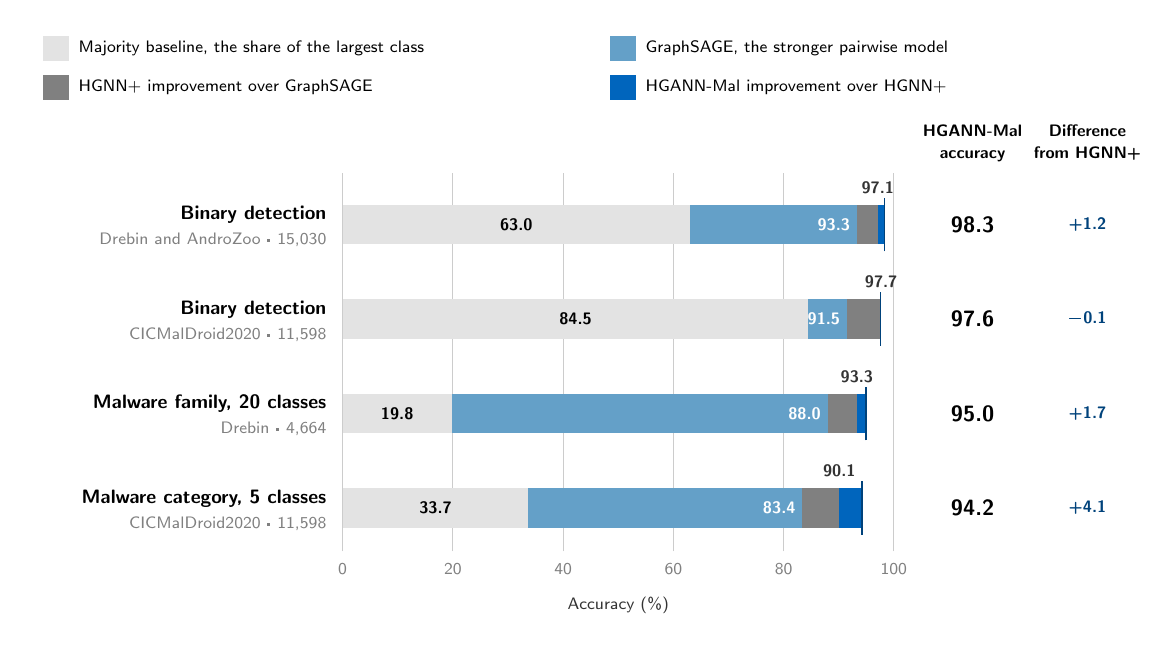
\begin{tikzpicture}[x=1mm,y=1mm]
  \useasboundingbox (0,0) rectangle (141.6,76);

  \legenditem{2}{73.4}{majority}{Majority baseline, the share of the largest class}
  \legenditem{74}{73.4}{tumblueii}{GraphSAGE, the stronger pairwise model}
  \legenditem{2}{68.4}{tumgrey}{HGNN+ improvement over GraphSAGE}
  \legenditem{74}{68.4}{tumblue}{HGANN-Mal improvement over HGNN+}

  \foreach \v in {0,20,40,60,80,100}{%
    \pgfmathsetmacro{\xx}{\accx{\v}}%
    \draw[tumgreylight,line width=0.3pt] (\xx,9.5) -- (\xx,57.5);
    \node[text=tumgrey,inner sep=0pt] at (\xx,7.2) {\axisfont \v};
  }
  \node[inner sep=0pt,text=tumgreydark] at (\accx{50},2.6) {\labelfont Accuracy (\%)};
  \node[anchor=base,inner sep=0pt] at (120,62.2) {\labelfont\bfseries HGANN-Mal};
  \node[anchor=base,inner sep=0pt] at (120,59.4) {\labelfont\bfseries accuracy};
  \node[anchor=base,inner sep=0pt] at (134.6,62.2) {\labelfont\bfseries Difference};
  \node[anchor=base,inner sep=0pt] at (134.6,59.4) {\labelfont\bfseries from HGNN+};

  \accrow{51}{Binary detection}{Drebin and AndroZoo \textperiodcentered{} 15,030}
    {63.0}{93.3}{97.1}{98.3}{+1.2}
  \accrow{39}{Binary detection}{CICMalDroid2020 \textperiodcentered{} 11,598}
    {84.5}{91.5}{97.7}{97.6}{\textminus 0.1}
  \accrow{27}{Malware family, 20 classes}{Drebin \textperiodcentered{} 4,664}
    {19.8}{88.0}{93.3}{95.0}{+1.7}
  \accrow{15}{Malware category, 5 classes}{CICMalDroid2020 \textperiodcentered{} 11,598}
    {33.7}{83.4}{90.1}{94.2}{+4.1}
\end{tikzpicture}
\end{document}
